\documentclass[tikz,border=10pt]{standalone}
\usepackage{tikz}
\usetikzlibrary{positioning, calc, arrows.meta, fit}

\begin{document}
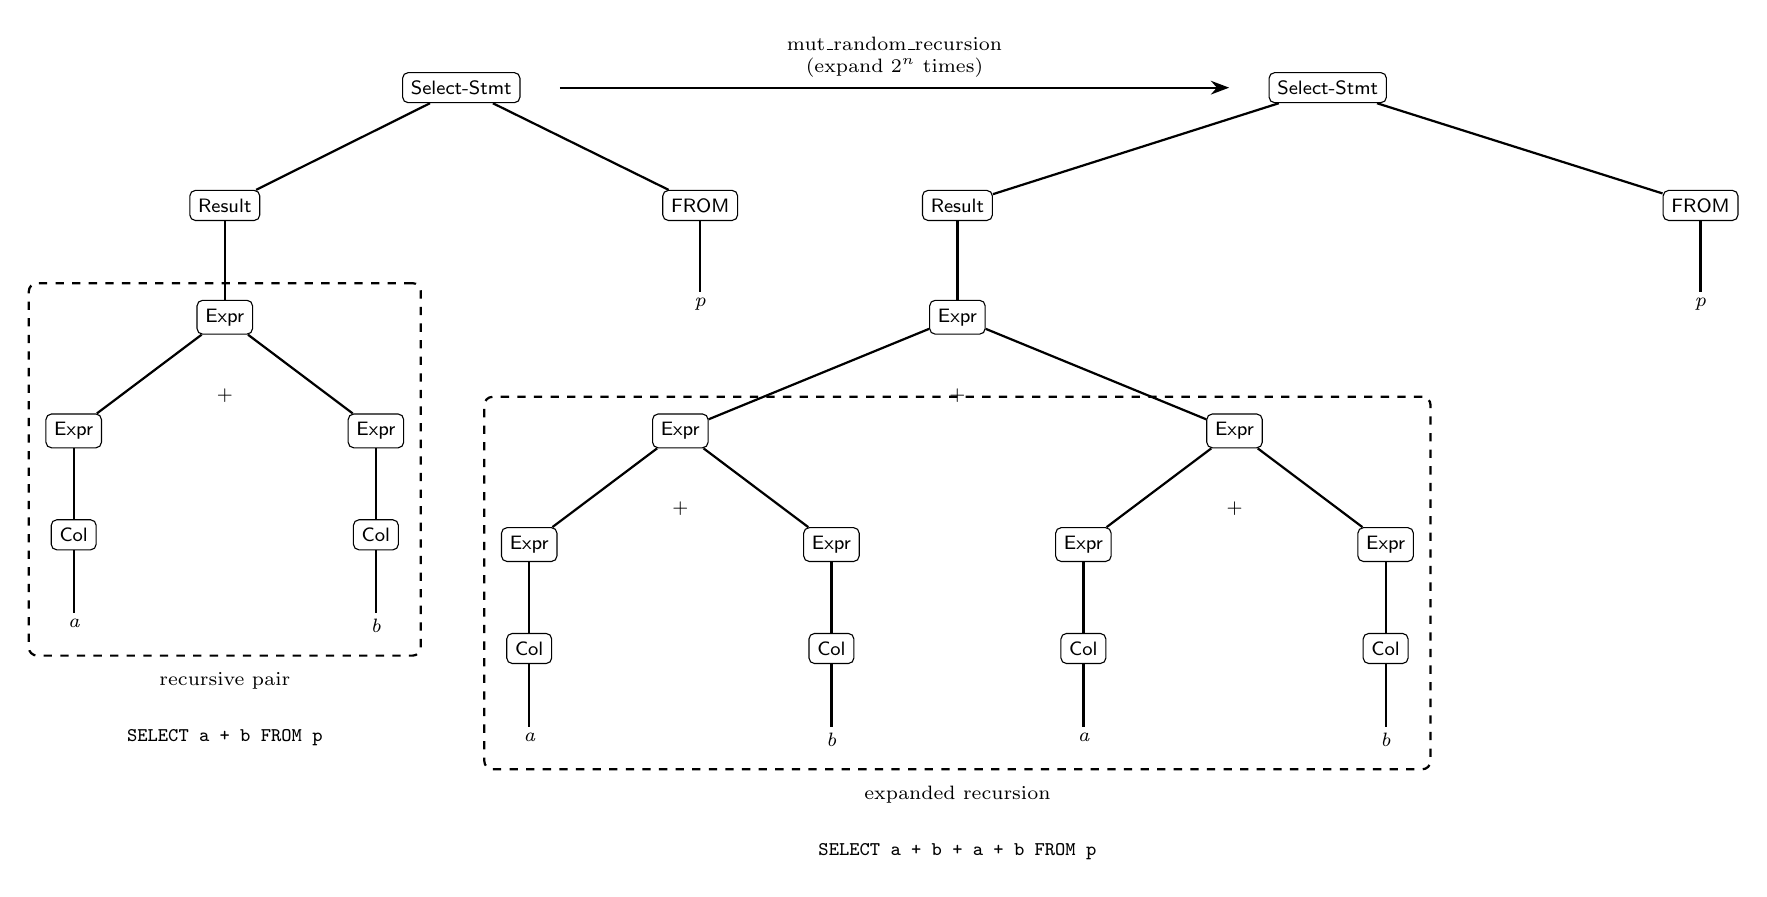
\begin{tikzpicture}[
    % Node styles
    nonterm/.style={
        draw, rounded corners=2pt, inner sep=3pt,
        font=\scriptsize\sffamily
    },
    term/.style={
        font=\scriptsize\itshape, inner sep=2pt
    },
    optext/.style={
        font=\scriptsize\sffamily, inner sep=1pt
    },
    % Edge style
    edge/.style={draw, thick},
    % Arrow style
    arrow/.style={-{Stealth[scale=1.0]}, thick},
    % Dashed box
    dashrect/.style={draw, dashed, thick, rounded corners=3pt, inner sep=6pt},
]

% ===== LEFT TREE (Before): SELECT a + b FROM p =====

% Root
\node[nonterm] (L-root) {Select-Stmt};

% Level 1: Result, FROM
\node[nonterm, below left=1.1cm and 1.8cm of L-root] (L-result) {Result};
\node[nonterm, below right=1.1cm and 1.8cm of L-root] (L-from) {FROM};

% Edges from root
\draw[edge] (L-root) -- (L-result);
\draw[edge] (L-root) -- (L-from);

% FROM child: p
\node[term, below=0.9cm of L-from] (L-p) {p};
\draw[edge] (L-from) -- (L-p);

% Level 2: Expr (under Result)
\node[nonterm, below=1.0cm of L-result] (L-expr) {Expr};
\draw[edge] (L-result) -- (L-expr);

% Level 3: Expr + Expr (children of top Expr)
\node[nonterm, below left=1.0cm and 1.2cm of L-expr] (L-el) {Expr};
\node[nonterm, below right=1.0cm and 1.2cm of L-expr] (L-er) {Expr};
\draw[edge] (L-expr) -- (L-el);
\draw[edge] (L-expr) -- (L-er);

% + operator label between children
\node[optext] at ($(L-el)!0.5!(L-er) + (0, 0.45)$) {+};

% Level 4: Col nodes
\node[nonterm, below=0.9cm of L-el] (L-col-a) {Col};
\node[nonterm, below=0.9cm of L-er] (L-col-b) {Col};
\draw[edge] (L-el) -- (L-col-a);
\draw[edge] (L-er) -- (L-col-b);

% Level 5: terminals a, b
\node[term, below=0.8cm of L-col-a] (L-a) {a};
\node[term, below=0.8cm of L-col-b] (L-b) {b};
\draw[edge] (L-col-a) -- (L-a);
\draw[edge] (L-col-b) -- (L-b);

% Dashed box around recursive pair (Expr -> Expr + Expr)
\node[dashrect, fit=(L-expr)(L-el)(L-er)(L-col-a)(L-col-b)(L-a)(L-b)] (L-box) {};
\node[font=\scriptsize, below=2pt of L-box.south, anchor=north] {recursive pair};

% SQL label
\node[font=\scriptsize\ttfamily, below=0.8cm of L-box.south, anchor=north] (L-sql)
    {\texttt{SELECT a + b FROM p}};


% ===== RIGHT TREE (After): SELECT a + b + a + b FROM p =====
% Shifted far to the right for generous spacing

% Root
\node[nonterm, right=9.5cm of L-root] (R-root) {Select-Stmt};

% Level 1: Result, FROM
\node[nonterm, below left=1.1cm and 3.5cm of R-root] (R-result) {Result};
\node[nonterm, below right=1.1cm and 3.5cm of R-root] (R-from) {FROM};

\draw[edge] (R-root) -- (R-result);
\draw[edge] (R-root) -- (R-from);

% FROM child: p
\node[term, below=0.9cm of R-from] (R-p) {p};
\draw[edge] (R-from) -- (R-p);

% Level 2: top Expr
\node[nonterm, below=1.0cm of R-result] (R-top) {Expr};
\draw[edge] (R-result) -- (R-top);

% Level 3: Expr + Expr (first split)
\node[nonterm, below left=1.0cm and 2.8cm of R-top] (R-left) {Expr};
\node[nonterm, below right=1.0cm and 2.8cm of R-top] (R-right) {Expr};
\draw[edge] (R-top) -- (R-left);
\draw[edge] (R-top) -- (R-right);

% + operator at top split
\node[optext] at ($(R-left)!0.5!(R-right) + (0, 0.45)$) {+};

% Level 4: Left branch splits into Expr + Expr
\node[nonterm, below left=1.0cm and 1.2cm of R-left] (R-ll) {Expr};
\node[nonterm, below right=1.0cm and 1.2cm of R-left] (R-lr) {Expr};
\draw[edge] (R-left) -- (R-ll);
\draw[edge] (R-left) -- (R-lr);

% + operator for left branch
\node[optext] at ($(R-ll)!0.5!(R-lr) + (0, 0.45)$) {+};

% Level 4: Right branch splits into Expr + Expr
\node[nonterm, below left=1.0cm and 1.2cm of R-right] (R-rl) {Expr};
\node[nonterm, below right=1.0cm and 1.2cm of R-right] (R-rr) {Expr};
\draw[edge] (R-right) -- (R-rl);
\draw[edge] (R-right) -- (R-rr);

% + operator for right branch
\node[optext] at ($(R-rl)!0.5!(R-rr) + (0, 0.45)$) {+};

% Level 5: Col nodes
\node[nonterm, below=0.9cm of R-ll] (R-col-a1) {Col};
\node[nonterm, below=0.9cm of R-lr] (R-col-b1) {Col};
\node[nonterm, below=0.9cm of R-rl] (R-col-a2) {Col};
\node[nonterm, below=0.9cm of R-rr] (R-col-b2) {Col};
\draw[edge] (R-ll) -- (R-col-a1);
\draw[edge] (R-lr) -- (R-col-b1);
\draw[edge] (R-rl) -- (R-col-a2);
\draw[edge] (R-rr) -- (R-col-b2);

% Level 6: terminal leaves
\node[term, below=0.8cm of R-col-a1] (R-a1) {a};
\node[term, below=0.8cm of R-col-b1] (R-b1) {b};
\node[term, below=0.8cm of R-col-a2] (R-a2) {a};
\node[term, below=0.8cm of R-col-b2] (R-b2) {b};
\draw[edge] (R-col-a1) -- (R-a1);
\draw[edge] (R-col-b1) -- (R-b1);
\draw[edge] (R-col-a2) -- (R-a2);
\draw[edge] (R-col-b2) -- (R-b2);

% Dashed box around expanded recursion level
\node[dashrect, fit=(R-left)(R-right)(R-ll)(R-lr)(R-rl)(R-rr)(R-col-a1)(R-col-b1)(R-col-a2)(R-col-b2)(R-a1)(R-b1)(R-a2)(R-b2)] (R-box) {};
\node[font=\scriptsize, below=2pt of R-box.south, anchor=north] {expanded recursion};

% SQL label
\node[font=\scriptsize\ttfamily, below=0.8cm of R-box.south, anchor=north] (R-sql)
    {\texttt{SELECT a + b + a + b FROM p}};


% ===== ARROW between trees =====
\draw[arrow] ([xshift=0.5cm]L-root.east)
    -- node[above, font=\scriptsize, align=center, text width=4.5cm]
    {mut\_random\_recursion\\(expand $2^n$ times)}
    ([xshift=-0.5cm]R-root.west);

\end{tikzpicture}
\end{document}
